\chapter{Finding the root cause}
\label{ch:rank}

\section{Step one: split a service's trouble into ``mine'' and ``inherited''}
\begin{simplebox}
Back to the restaurant. The waiter is unhappy because the kitchen is slow. The waiter's unhappiness is real, but it is \emph{explained by the kitchen}. If you ask ``whose fault is it?'' you do not want to point at the waiter.

For each service we ask: is its trouble coming from its \emph{own} resources (its CPU is maxed out, its memory is full), or is it showing only \emph{symptoms} (slow responses, errors, odd traffic) that could simply be inherited from something it calls? CPU, memory and throttling are \emph{own} signals, because a dependency cannot make your CPU spin. Traffic, errors, latency and network are \emph{symptoms}, because you can inherit them. If a service's symptoms are fully explained by a sick service it depends on, we subtract that explanation. What is left is the service's own contribution.
\end{simplebox}

\begin{techbox}
With own level $o(s)$, symptom level $\sigma(s)$ and callees $C(s)$,
\begin{align*}
x(s)&=\gamma\max_{c\in C(s)}a(c),\\
\operatorname{raw}(s)&=\max\bigl(o(s),\ \max(0,\ \sigma(s)-x(s))\bigr),
\end{align*}
where $a(c)$ is the anomaly level of a callee and $\gamma=1.0$ is the weight of what a sick callee explains. A service whose symptoms a sick callee fully explains drops out; one that is abnormal in its own resources stays. The ML engine keeps the two levels (own and symptom) separate for exactly this purpose.
\end{techbox}

\begin{examplebox}[Worked example: three services in a chain]
\code{checkout}\,$\to$\,\code{orders}\,$\to$\,\code{orders-db}. The database's disk is the real problem. Levels right now (1.0 = the service's own alarm line):

\medskip
\begin{center}
\small
\begin{tabular}{lrrr}
\toprule
Service & own level $o$ & symptom level $\sigma$ & what its callee explains $x$\\
\midrule
orders-db & 2.5 & 0.5 & (none, it has no callee) \\
orders & 0.1 & 2.2 & $1.0\times\max(a_{\text{orders-db}})\approx 2.5$\\
checkout & 0.0 & 1.8 & $1.0\times\max(a_{\text{orders}})\approx 2.2$\\
\bottomrule
\end{tabular}
\end{center}

Then $\operatorname{raw}(\text{orders-db})=\max(2.5,\ \max(0,0.5-0))=2.5$. For \code{orders}: $\max(0.1,\ \max(0,2.2-2.5))=0.1$. For \code{checkout}: $\max(0.0,\ \max(0,1.8-2.2))=0.0$. Even though \code{orders} and \code{checkout} are loud (symptoms 2.2 and 1.8), their trouble is explained by the service they call, so they drop to nearly zero. \code{orders-db} keeps 2.5. It is ranked first.
\end{examplebox}

\section{Step two: the random walk}
\begin{simplebox}
The first step is local: it looks at each service and its neighbours. The second step looks at the \emph{whole map}. Imagine a little walker standing on the map. At each step it moves along a link, but it prefers to move toward services that look abnormal and it likes to stay on a service whose trouble nothing downstream explains. Now let the walker walk for a very long time and count how much time it spent at each service. The service it visits the most is the best candidate for the origin. Why? Trouble flows \emph{toward} callers, so the walker following the trail of trouble ends up circling the place it started from.

This idea is a classic (it is the same maths as Google's original PageRank, adapted to a call graph). We did not invent it. We feed it better inputs.
\end{simplebox}

\begin{techbox}
The ranker is a personalised-PageRank walk in the MonitorRank form. A walker on the directed graph steps to a callee $v$ with weight $w(u\to v)\,a(v)$, back to a caller with weight $\rho_{\mathrm b}\,a(u)$, and stays with weight $\max(0,\ a(u)-\max_c a(c),\ o(u))$, restarting on the anomalous set with probability $\alpha=0.15$. The stationary share $\pi_s$ is the score, and services with a container fact rank first. The \emph{stay} term is what lets the true source, whose trouble nothing downstream explains, collect the most mass. The edge weights $w(e)$ are the evidence-weighted confidences of Part~\ref{ch:graph}.
\end{techbox}

\begin{saybox}
``The decomposition removes inherited trouble locally; the random walk then combines that over the whole graph. And facts rank first, because a stopped container is a certainty.''
\end{saybox}

\section{What the evidence says about ranking}
\begin{center}
\small
\begin{tabular}{lcccc}
\toprule
Ranking method (real systems, 62 faults) & C+N & 95\% CI & A@1 & A@3\\
\midrule
Rules & 63 & [52, 74] & 70 & 91\\
Severity (loudest service) & 68 & [56, 79] & 75 & 86\\
ML (load model + walk) & 71 & [60, 81] & 79 & 89\\
Hybrid (default) & 71 & [60, 81] & 79 & 89\\
\bottomrule
\end{tabular}
\end{center}

\begin{simplebox}
\textbf{A@1} is: among the faults we detected, how often was the true root cause ranked first? \textbf{A@3} is: how often was it in the top three? \textbf{C+N} is: out of \emph{all} faults, how often did we detect it \emph{and} rank it first? The bracket is the range in which the true rate probably lies (a 95\% confidence interval).

The interesting part is that the walk is \emph{not} significantly better than just ranking by the loudest anomaly. The difference between Hybrid and Rules is $+8.1$ points with an interval of $[-1.6,+17.7]$ and $p=0.117$. We report this honestly.
\end{simplebox}

\subsection{When does the graph matter? The amplification study}
\begin{simplebox}
In most of our faults the broken service is also the loudest service, so a naive ``loudest first'' wins. That tells you nothing about the graph. To test the case where the graph \emph{should} matter, we made a version where victims get louder than the origin (like a retry storm). We turned up the ``amplification'' knob from 1 (normal) to 4 (victims feel it four times as hard). If the graph logic is worth anything, ranking by the walk should hold up while ranking by loudness should fall.
\end{simplebox}

\begin{figure}[H]
\centering
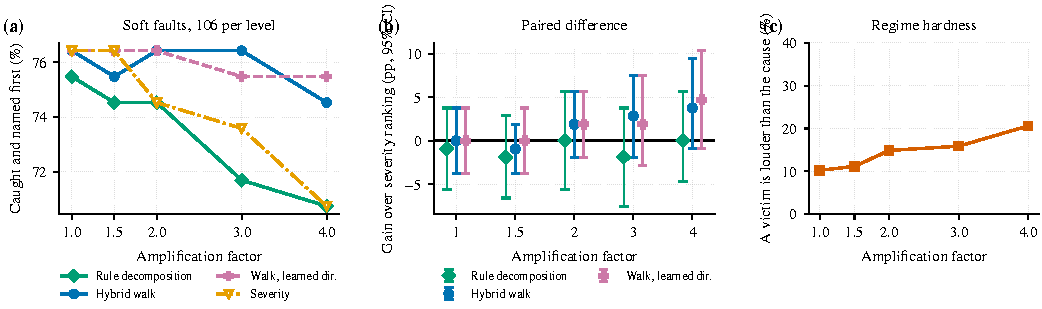
\includegraphics[width=0.98\textwidth]{fig_amp.pdf}
\caption{Amplification study on soft faults (106 per level).}
\end{figure}

\begin{techbox}
Soft faults (brownout, latency, memory) were regenerated with the amplification factor $A\in\{1,1.5,2,3,4\}$, the hybrid's alarms were kept identical for every ranker and only the ranking varied. As $A$ grows, the share of faults in which some victim is louder than the true cause rises from 10\% to 21\%, the severity ranking falls from 76\% to 71\%, and the walk holds at 75--76\%, so the gain of the walk over severity grows from zero to $+3.8$ points (95\% CI $[-0.9,+9.4]$ at $A=4$) and that of the walk with learned directions to $+4.7$ ($[-0.9,+10.4]$). The intervals include zero at every level. So the shape is as the theory predicts, but the sample is too small to confirm it.
\end{techbox}

\begin{warnbox}
Do not claim ``the graph ranking is proven better''. Say ``it behaves as theory predicts as amplification grows, the gain is a few points, and our sample is too small to confirm it''.
\end{warnbox}

\section{Per-class accuracy: where it works and where it does not}
\begin{figure}[H]
\centering
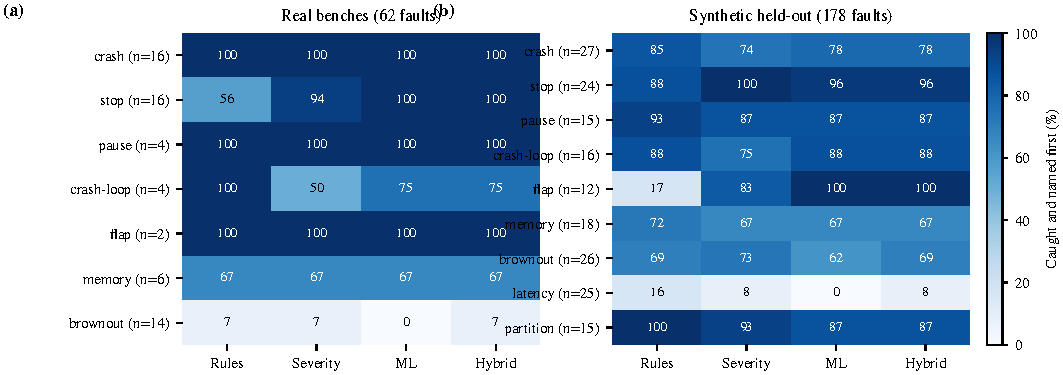
\includegraphics[width=0.98\textwidth]{fig_class.pdf}
\caption{Caught-and-named rate by fault class (percent; $n$ faults per class), on the real systems (a) and the synthetic held-out set (b).}
\end{figure}

\begin{simplebox}
The tool is best at faults with a clear \emph{fact} (a container that stops or is paused) and weakest at \emph{brownouts}: a service that is slowed down by a resource limit but not stopped, especially when it was nearly idle to begin with. A nearly idle service that gets slower barely changes any of the eight numbers, so there is nothing for any detector to see. That is an honest open problem; we show it on the figure and say it in the limitations.
\end{simplebox}
